\section{XY for Previously seen Queries}

Our approach.

We noticed that queries overlap over different time slots, and in case their intent stays the same, we aim to transfer their relevance information to the new time slots. Consecutively, for those queries we know what documents were clicked a few months ago. We decided to use this feedback and query expansion with the BO1 model~\cite{amati:2003} to create keyqueries and use the same approach as \cite{froebe-mis:2022}. Thereby, we use BO1 to obtain candidate terms for query terms, as pilot experiments showed that BO1 expansion terms yield higher effectiveness than RM3~\cite{jaleel:2004} expansions. We inserted the clicked documents into the current corpus and reformulated the queries with the BO1 model until those documents were in the top positions. After that we removed old documents from the ranking. This implementation of the keyquery concept is not the most effective one, more effective approaches that leverage a generate-and-test paradigm~\cite{froebe:2021c} exist and are interesting directions for future work (i.e., explicitly generating many variants and selecting the variants that are highly effective).

Short analysis: how much did documents change? We use CopyCat~\cite{froebe:2021a}, as it was previously used to deduplicate web crawls, e.g., the ClueWebs, in default settings. ToDo: add motivation for measure and containment conceptually implemented by the S3 score.

\begin{figure}[t]
    \begin{minipage}{.49\textwidth}
        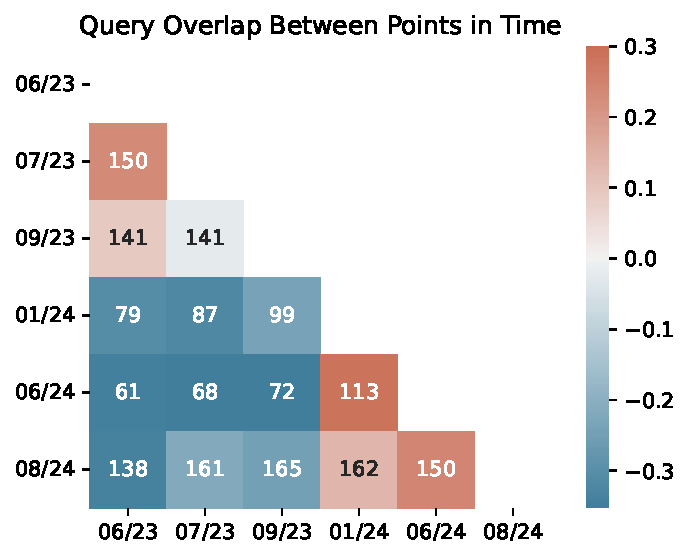
\includegraphics[width=\textwidth]{query-overlap}
        \vspace{-4ex}
        \caption{Frequency of queries and points in time.}
        \label{fig:query-overlap}
    \end{minipage}
    \hfill    
    \begin{minipage}{.49\textwidth}
        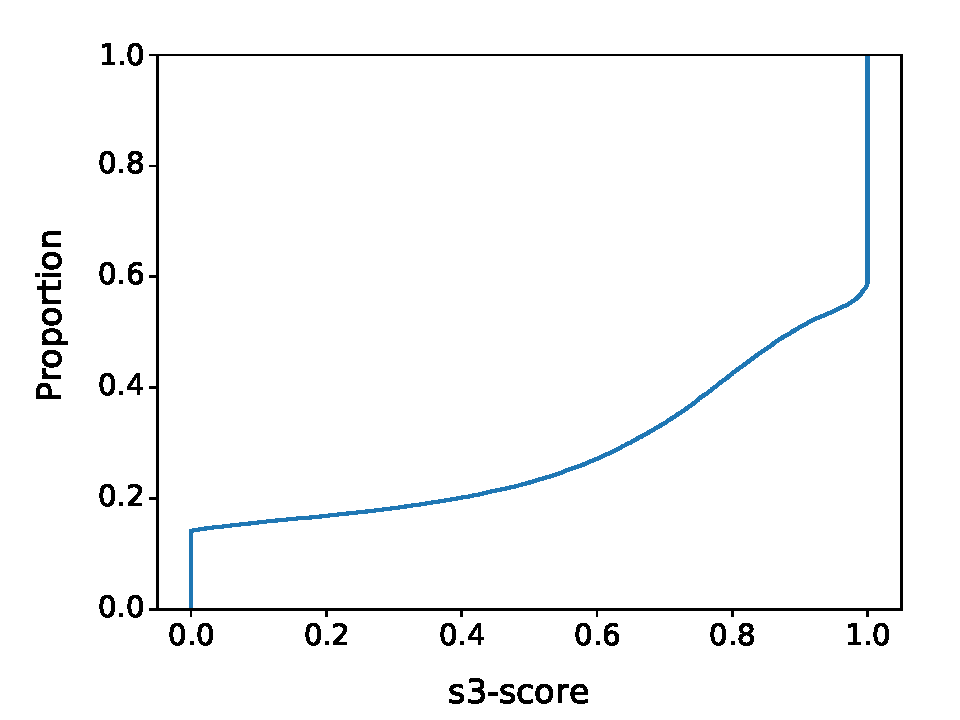
\includegraphics[width=\textwidth]{document-similarities}
        \vspace{-4ex}
        \caption{S$_{3}$ Similarities of documents with overlapping URLs as eCDF plot.}
        \label{fig:document-similarities}
    \end{minipage}
\end{figure}